\documentclass[11pt]{standalone}
\usepackage[T1]{fontenc}
\usepackage{tikz}
\usetikzlibrary{calc,positioning,shapes.geometric}

\begin{document}
  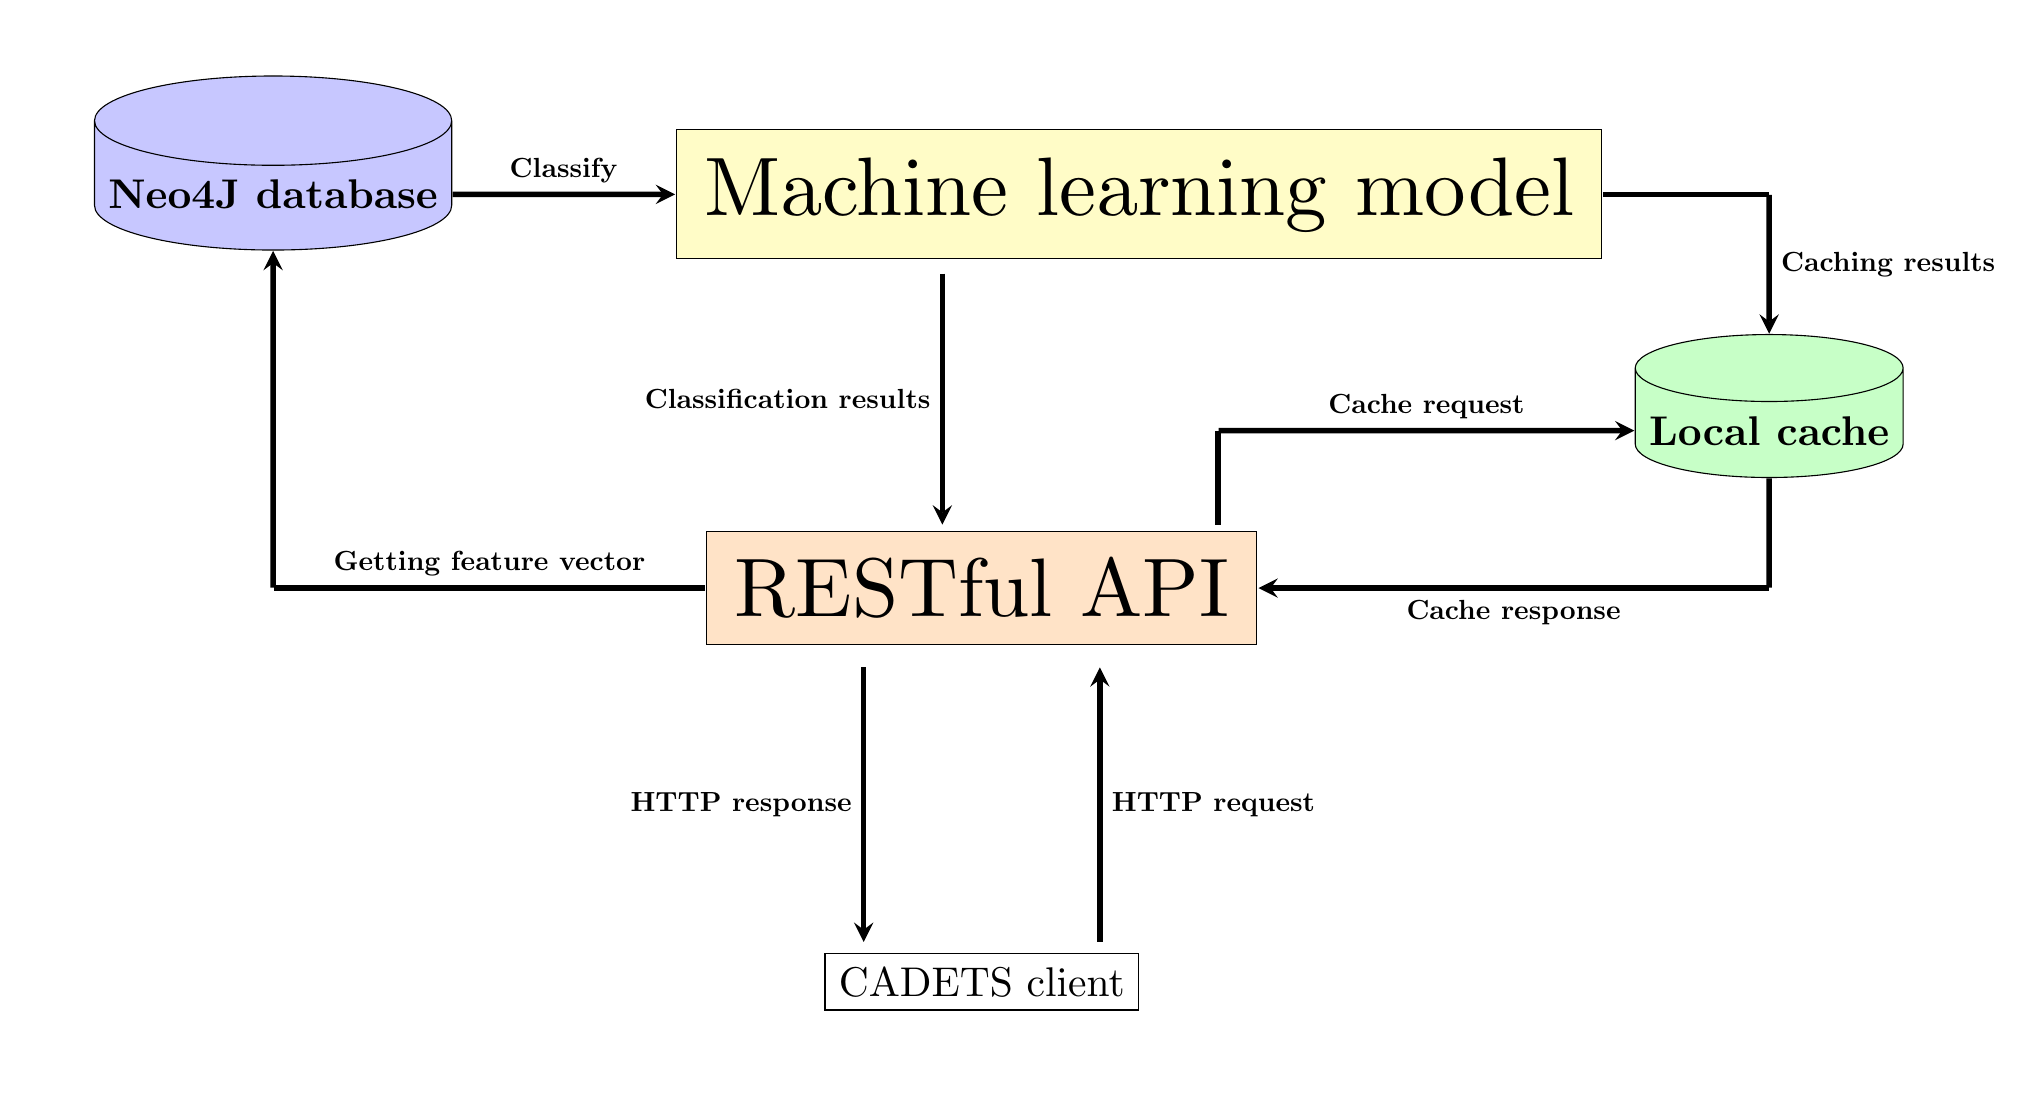
\begin{tikzpicture}[
    >=stealth,
    node distance=3cm,
    database/.style={
      cylinder,
      cylinder uses custom fill,
      cylinder body fill=yellow!50,
      cylinder end fill=yellow!50,
      shape border rotate=90,
      aspect=0.25,
      scale=1.5,
      draw
    },
	rectangle-REST/.style={
		rectangle,
		aspect=0.25,
		scale=3,
		draw
	},
  ]
  
  %%%%%%%%%%%%%%%%%%%%%%%%%%%%%%%%%%%%%%%%%%%%%%
  %%%%%%%%%%%%%%%% ACTUAL NODES %%%%%%%%%%%%%%%%%%%
   %%%%%%%%%%%%%%%%%%%%%%%%%%%%%%%%%%%%%%%%%%%%%%
    \node[database, fill=blue!22] (Neo4J) at (1,10) {\textbf{Neo4J database}};
    \node[database, fill=green!22] (cache) at (20,7) {\textbf{Local cache}};
   
    \node[rectangle-REST, fill=orange!22] (REST) at (10,5) {RESTful API};
    
    \node[rectangle-REST, scale=.5] (CLIENT) at (10,0) {CADETS client};
    
    %\node[rectangle-REST, scale=.5] (features) at (6, 7) {Features collector};

	\node[rectangle-REST, fill=yellow!22] (ml) at (12, 10) {Machine learning model};

	%%%%%%%%%%%%%%%%%%%%%%%%%%%%%%%%%%%%%%%%%%%%%%
	%%%%%%%%%%%%%%%% HELPING NODES %%%%%%%%%%%%%%%%%%%
	%%%%%%%%%%%%%%%%%%%%%%%%%%%%%%%%%%%%%%%%%%%%%%
	\node at (-2,12)  {};
	\node at (22,-1)  {};
	
	\node[scale=.05] (cache-REST) at (20, 5) {};
	\node[scale=.05] (REST-cache) at (13, 7) {};
	\node[scale=0.05] (REST-cache-REST) at (13, 5.8) {};
	
	\node[scale=.05] (features-neo4j) at (1, 7) {};
	\node[scale=.05] (neo4j-features) at (4.5, 10) {};
	\node[scale=.05] (neo4j-features-features) at (4.5, 7.4) {};
	
	\node[scale=.05] (REST-client-client) at (8.5, 0.5) {};
	\node[scale=.05] (REST-client-REST) at (8.5, 4) {};
	
	\node[scale=.05] (client-REST-client) at (11.5, 0.5) {};
	\node[scale=.05] (client-REST-REST) at (11.5, 4) {};
	
	\node[scale=.05] (REST-features-features) at (6.5, 6.6) {};
	\node[scale=.05] (REST-features-REST) at (6.5, 5.8) {};
	
	\node[scale=0.05] (features-ml-features) at (8, 7.4) {};
	\node[scale=0.05] (features-ml-ml) at (8, 9) {};
	
	\node[scale=0.05] (ml-REST-ml) at (9.5, 9) {};
	\node[scale=0.05] (ml-REST-REST) at (9.5, 5.8) {};
	
	\node[scale=0.05] (ml-cache) at (20, 10) {};
	
	\node[scale=0.05] (REST-neo4j) at (1, 5) {};

	%%%%%%%%%%%%%%%%%%%%%%%%%%%%%%%%%%%%%%%%%%%%%%
	%%%%%%%%%%%%%%%%%% PATHS %%%%%%%%%%%%%%%%%%%%%%%
	%%%%%%%%%%%%%%%%%%%%%%%%%%%%%%%%%%%%%%%%%%%%%%
	
	\path [-, draw, line width = 2pt] (cache) -- (cache-REST) {};
	\path [->, draw, line width = 2pt] (cache-REST) -- (REST) node[below, midway] {\textbf{Cache response}};
	
	\path [-, draw, thick, line width = 2pt] (REST-cache-REST) -- (REST-cache) {};
	\path [->, draw, thick, line width = 2pt] (REST-cache) -- (cache) node[above, midway] {\textbf {Cache request}};
	
	%\path [-, draw, thick] (features) -- (features-neo4j) {};
	%\path [->, draw, thick] (features-neo4j) -- (Neo4J) node[left, midway] {Features request};
	
	%\path [-, draw, thick] (Neo4J) -- (neo4j-features) {};
	%\path [->, draw, thick] (neo4j-features) -- (neo4j-features-features) node[left, midway] {Features response};
	
	\path [->, draw, line width = 2pt] (REST-client-REST) -- (REST-client-client) node[left, midway] {\textbf{HTTP response}};
	\path [->, draw, line width = 2pt] (client-REST-client) -- (client-REST-REST) node[right, midway] {\textbf{HTTP request}};
    
    %\path[->, draw, thick] (REST-features-REST) -- (REST-features-features) {};
    
    %\path[->, draw, thick] (features-ml-features) -- (features-ml-ml) node[left, midway] {Classification};
    
    \path[->, draw, line width = 2pt] (ml-REST-ml) -- (ml-REST-REST) node[left, midway] {\textbf{Classification results}};
    
    \path [-, draw, line width = 2pt] (ml) -- (ml-cache) {};
    \path [->, draw, line width = 2pt] (ml-cache) -- (cache) node[right, midway] {\textbf{Caching results}};
     
    \path[-, draw, line width = 2pt] (REST) -- (REST-neo4j) node[above, midway] {\textbf{Getting feature vector}};
    \path[->, draw, line width = 2pt] (REST-neo4j) -- (Neo4J) {};
    
    \path[->, draw, line width = 2pt] (Neo4J) -- (ml) node[above, midway] {\textbf{Classify}};
    
  \end{tikzpicture}
\end{document}